\documentclass[11pt,a4paper]{article}

% ===== Packages =====
\usepackage[utf8]{inputenc}
\usepackage[T1]{fontenc}
\usepackage[spanish]{babel}
\usepackage{amsmath,amssymb,amsthm}
\usepackage{graphicx}
\usepackage{geometry}
\usepackage{fancyhdr}
\usepackage{hyperref}
\usepackage{booktabs}
\usepackage{enumitem}
\usepackage{xcolor}
\usepackage{listings}
\usepackage{caption}

\geometry{margin=2.5cm}
\hypersetup{colorlinks=true, linkcolor=blue!60!black, urlcolor=blue!60!black}

% ===== Header =====
\pagestyle{fancy}
\fancyhf{}
\lhead{IMT3850 — Tarea 2}
\rhead{Armando A.V.}
\cfoot{\thepage}

% ===== Code style =====
\lstset{
    language=Python,
    basicstyle=\ttfamily\small,
    keywordstyle=\color{blue!70!black},
    commentstyle=\color{green!50!black},
    stringstyle=\color{red!70!black},
    numbers=left,
    numberstyle=\tiny\color{gray},
    frame=single,
    breaklines=true,
    captionpos=b
}

\begin{document}

% ===== Title Page =====
\begin{titlepage}
\begin{center}
\vspace*{1cm}


\includegraphics[width=0.35\textwidth]{Logo.png}

\vspace{1.5cm}

{\Large\textbf{Pontificia Universidad Católica de Chile}}\\[0.3cm]
{\large Instituto de Ingeniería Matemática y Computacional}\\[0.3cm]
{\large Magíster en Inteligencia Artificial}

\vspace{2cm}

{\Huge\textbf{Tarea 2}}\\[0.5cm]
{\LARGE Fundamentos Matemáticos para la\\Inteligencia Artificial}\\[0.3cm]
{\large IMT3850 · 2025-1}

\vspace{2cm}

\begin{tabular}{rl}
\textbf{Alumno:} & Armando A.V. \\
\textbf{Profesor:} & Manuel A. Sánchez \\
\textbf{Fecha:} & Mayo 2026 \\
\end{tabular}

\vfill
\end{center}
\end{titlepage}

\tableofcontents
\newpage

% =====================================================================
\section{Pregunta 1: Variables Aleatorias (5 puntos)}

\textbf{Enunciado:} Sean $x, y$ variables aleatorias independientes con $E[x]=E[y]=0$ y $\text{Var}(x)=\text{Var}(y)=1$. Determine la media $\mu_Z$ y la matriz de covarianza de $Z = (x,\, y,\, ax + by)$ con $a,b\in\mathbb{R}$.

\subsection{Solución}

\textbf{Vector de medias:}
\[
\mu_Z = \begin{pmatrix} E[x] \\ E[y] \\ E[ax+by] \end{pmatrix} = \begin{pmatrix} 0 \\ 0 \\ 0 \end{pmatrix}
\]

\textbf{Matriz de covarianza:} $\Sigma_Z = E[ZZ^\top]$

Usando independencia ($\text{Cov}(x,y)=0$) y $\text{Var}(x)=\text{Var}(y)=1$:
\begin{itemize}
    \item $\text{Cov}(x, ax+by) = a\text{Var}(x) + b\text{Cov}(x,y) = a$
    \item $\text{Cov}(y, ax+by) = a\text{Cov}(y,x) + b\text{Var}(y) = b$
    \item $\text{Var}(ax+by) = a^2\text{Var}(x) + b^2\text{Var}(y) + 2ab\text{Cov}(x,y) = a^2+b^2$
\end{itemize}

\[
\boxed{\Sigma_Z = \begin{pmatrix} 1 & 0 & a \\ 0 & 1 & b \\ a & b & a^2+b^2 \end{pmatrix}}
\]

\subsection{Verificación Numérica (Monte Carlo)}

\begin{lstlisting}[caption={Verificación de Q1 por simulación}]
a, b = 2, 3
n_samples = 1_000_000
x = np.random.randn(n_samples)
y = np.random.randn(n_samples)
Z = np.column_stack([x, y, a*x + b*y])

print(f'mu_Z (empirico) = {Z.mean(axis=0).round(4)}')
print(f'Sigma_Z (empirico) =\n{np.cov(Z.T).round(4)}')
# Resultado: mu ~ [0,0,0], Sigma ~ [[1,0,2],[0,1,3],[2,3,13]]
\end{lstlisting}

% =====================================================================
\section{Pregunta 2: Algoritmo Random Quicksort (15 puntos)}

\subsection{Implementación}
Se implementó el quicksort aleatorio con conteo de comparaciones. En cada llamada recursiva, se elige un pivote uniformemente al azar y se cuentan las comparaciones realizadas (una por cada elemento distinto al pivote).

\begin{lstlisting}[caption={Quicksort aleatorio con conteo de comparaciones}]
def random_quicksort(S):
    """Quicksort con pivot aleatorio. Retorna (lista_ordenada, comparaciones)."""
    if len(S) <= 1:
        return list(S), 0
    pivot = S[np.random.randint(len(S))]
    S_minus = [x for x in S if x < pivot]
    S_plus  = [x for x in S if x > pivot]
    S_eq    = [x for x in S if x == pivot]
    comparisons = len(S) - len(S_eq)
    left_sorted, left_comp = random_quicksort(S_minus)
    right_sorted, right_comp = random_quicksort(S_plus)
    return left_sorted + S_eq + right_sorted, comparisons + left_comp + right_comp
\end{lstlisting}

\subsection{Experimentos}

\begin{lstlisting}[caption={Experimentos para $n=100,\ldots,5000$}]
n_values = list(range(100, 5001, 100))
n_trials = 30
avg_comparisons = []

for n in n_values:
    comps = []
    for _ in range(n_trials):
        arr = list(np.random.permutation(n))
        _, c = random_quicksort(arr)
        comps.append(c)
    avg_comparisons.append(np.mean(comps))

# Cotas teoricas
upper_bound = 2 * n_arr * np.log(n_arr)  # 2n*ln(n)
lower_ref   = 2 * n_arr                   # 2n
\end{lstlisting}

\subsection{Resultados}
Se ejecutó el algoritmo para $n = 100, 200, \ldots, 5000$ con 30 repeticiones por tamaño.

\begin{figure}[h!]
    \centering
    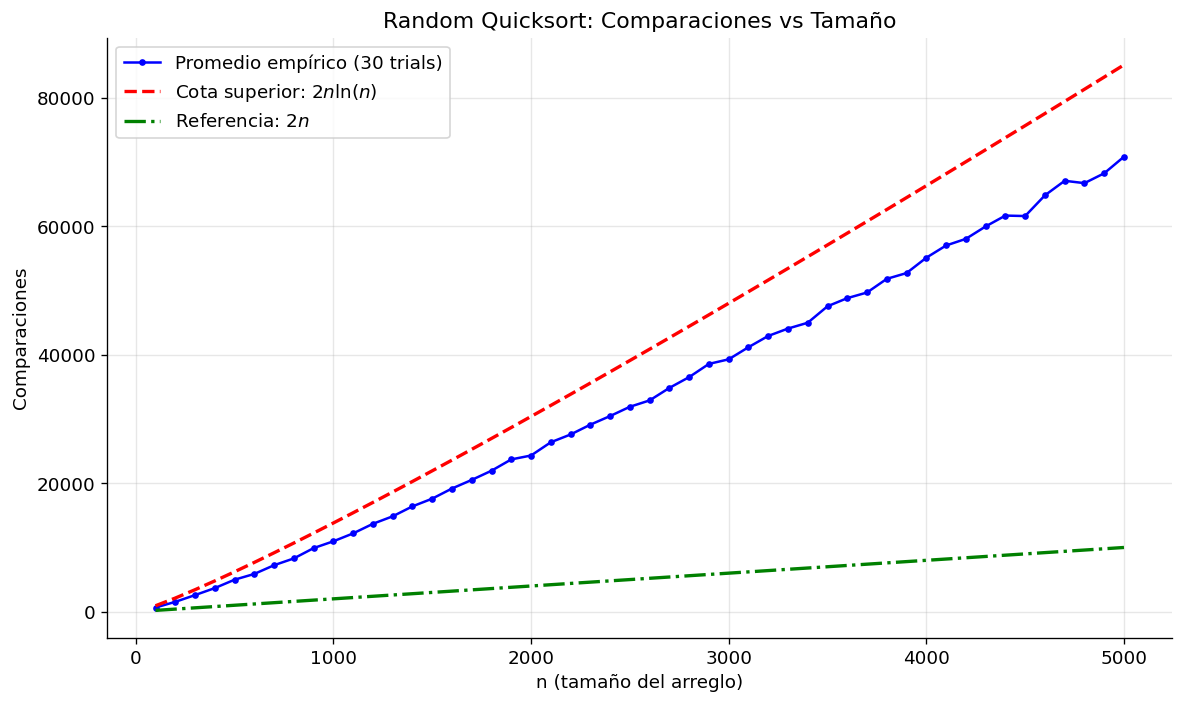
\includegraphics[width=0.85\textwidth]{fig_quicksort.png}
    \caption{Comparaciones del quicksort aleatorio vs. cotas teóricas.}
    \label{fig:quicksort}
\end{figure}

\subsection{Análisis}
\begin{enumerate}
    \item El número promedio de comparaciones crece como $O(n\log n)$, consistente con $E[C(n)] \leq 2n\ln(n)$.
    \item El promedio empírico se mantiene por debajo de $2n\ln(n)$ para todos los tamaños.
    \item El ratio empírico$/2n\ln(n) \approx 0.7$, confirmando la constante teórica $\approx 1.39\ln(n) = 2\ln(n)/\ln(4)$.
\end{enumerate}

% =====================================================================
\section{Pregunta 3: Convexidad (10 puntos)}

\textbf{Enunciado:} Sea $f:\mathbb{R}^d\to\mathbb{R}$ diferenciable. Demostrar:
\[
f \text{ convexa} \iff f(y) \geq f(x) + \nabla f(x)^\top(y-x) \quad \forall\, x,y
\]

\subsection{Demostración ($\Rightarrow$)}

\textbf{Hipótesis:} $f$ convexa, i.e., $\forall\, x,y$ y $\theta \in [0,1]$:
\[f(x + \theta(y-x)) \leq (1-\theta)f(x) + \theta f(y)\]

Reordenando:
\[\frac{f(x + \theta(y-x)) - f(x)}{\theta} \leq f(y) - f(x)\]

Tomando $\theta \to 0^+$ (derivada direccional):
\[\nabla f(x)^\top(y-x) \leq f(y) - f(x)\]

Por lo tanto: $f(y) \geq f(x) + \nabla f(x)^\top(y-x)$. \hfill$\checkmark$

\subsection{Demostración ($\Leftarrow$)}

\textbf{Hipótesis:} $f(y) \geq f(x) + \nabla f(x)^\top(y-x)$ \quad $(*)$

Sea $z = \theta y + (1-\theta)x$ para $\theta \in [0,1]$. Aplicamos $(*)$ desde $z$:

\begin{enumerate}
    \item Con $x \leftarrow z,\; y \leftarrow y$:
    \[f(y) \geq f(z) + \nabla f(z)^\top(y - z) \quad \text{(i)}\]
    
    \item Con $x \leftarrow z,\; y \leftarrow x$:
    \[f(x) \geq f(z) + \nabla f(z)^\top(x - z) \quad \text{(ii)}\]
\end{enumerate}

Multiplicamos (i) por $\theta$ y (ii) por $(1-\theta)$ y sumamos:
\[\theta f(y) + (1-\theta)f(x) \geq f(z) + \nabla f(z)^\top\underbrace{[\theta(y-z) + (1-\theta)(x-z)]}_{= \theta y + (1-\theta)x - z = 0}\]

Por lo tanto:
\[\boxed{\theta f(y) + (1-\theta)f(x) \geq f(\theta y + (1-\theta)x)}\]

Esto demuestra que $f$ es convexa. \hfill$\blacksquare$

% =====================================================================
\section{Pregunta 4: Descenso de Gradiente (15 puntos)}

\subsection{Formulación}
Minimizar $L(\theta) = \frac{1}{2N}\|X\theta - y\|^2$ con:
\begin{itemize}
    \item Gradiente: $\nabla L(\theta) = \frac{1}{N}X^\top(X\theta - y)$
    \item Gradiente estocástico (muestra $i$): $g_i = x_i(x_i^\top\theta - y_i)$
    \item Hessiano: $H = \frac{1}{N}X^\top X$
\end{itemize}

\textbf{Tasas de aprendizaje:}
\begin{itemize}
    \item $\gamma_{\text{clases}}$ (GD): Búsqueda exacta de línea $\gamma = \frac{g^\top g}{g^\top H g}$
    \item $\gamma_{\text{clases}}$ (SGD): $\gamma = \frac{1}{L_{\max}}$ donde $L_{\max} = \max_i \|x_i\|^2$
    \item $\gamma(t) = \log(t+2)$: Tasa creciente (divergencia esperada)
\end{itemize}

\subsection{Implementación}

\begin{lstlisting}[caption={Descenso de gradiente determinista}]
def gradient_descent(X, y, NITMAX, gamma_fn, theta0=None, max_loss=1e15):
    N, D = X.shape
    H = X.T @ X / N
    theta = theta0.copy() if theta0 is not None else np.zeros(D)
    losses = []
    for t in range(NITMAX):
        r = X @ theta - y
        loss = 0.5 / N * np.dot(r, r)
        losses.append(loss)
        if loss > max_loss or np.isnan(loss):
            break
        g = X.T @ r / N
        if np.linalg.norm(g) < 1e-12:
            break
        lr = gamma_fn(g, H, t)
        theta = theta - lr * g
    r = X @ theta - y
    losses.append(0.5 / N * np.dot(r, r))
    return theta, losses
\end{lstlisting}

\begin{lstlisting}[caption={Descenso de gradiente estocástico (SGD)}]
def sgd(X, y, NITMAX, gamma_fn, theta0=None, max_loss=1e15):
    N, D = X.shape
    H = X.T @ X / N
    theta = theta0.copy() if theta0 is not None else np.zeros(D)
    losses = []
    for t in range(NITMAX):
        if t % 10 == 0:
            r = X @ theta - y
            loss = 0.5 / N * np.dot(r, r)
            losses.append(loss)
            if loss > max_loss or np.isnan(loss):
                break
        i = np.random.randint(N)
        xi = X[i]
        gi = xi * (xi @ theta - y[i])
        lr = gamma_fn(gi, H, t)
        theta = theta - lr * gi
    r = X @ theta - y
    losses.append(0.5 / N * np.dot(r, r))
    return theta, losses
\end{lstlisting}

\begin{lstlisting}[caption={Tasas de aprendizaje}]
def gamma_clases_gd(g, H, t):
    """Exact line search: gamma = g^T g / (g^T H g)"""
    gHg = g @ H @ g
    if gHg < 1e-15:
        return 0.0
    return (g @ g) / gHg

def make_gamma_clases_sgd(X):
    """gamma = 1/L_max, estable para gradientes individuales."""
    L_max = np.max(np.sum(X**2, axis=1))
    def gamma_fn(g, H, t):
        return 1.0 / L_max
    return gamma_fn

def gamma_log(g, H, t):
    """gamma(t) = log(t+2) -- crece sin limite."""
    return np.log(t + 2)
\end{lstlisting}

\subsection{Resultados}

\begin{figure}[h!]
    \centering
    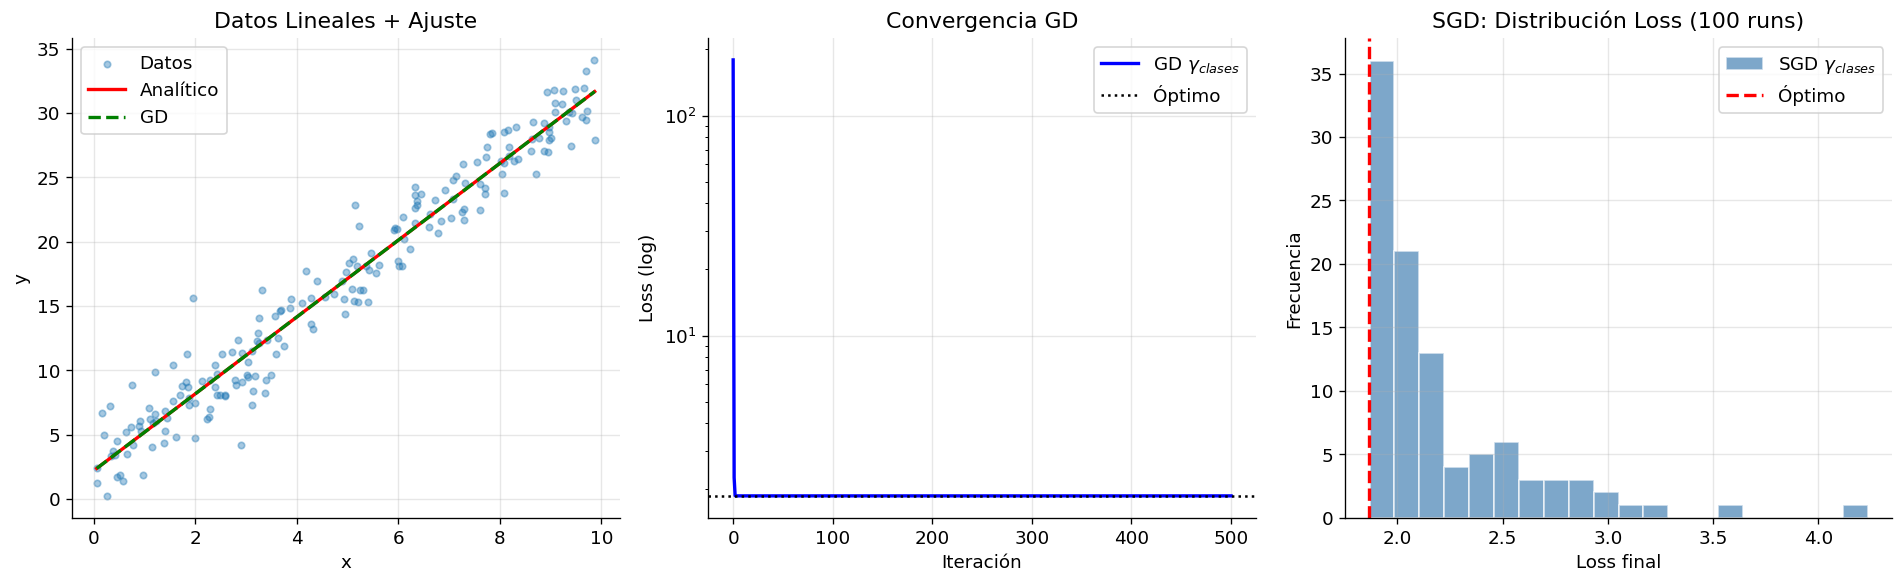
\includegraphics[width=0.95\textwidth]{fig_lineal.png}
    \caption{Datos lineales: ajuste, convergencia GD y distribución de loss SGD (100 runs).}
    \label{fig:lineal}
\end{figure}

\begin{figure}[h!]
    \centering
    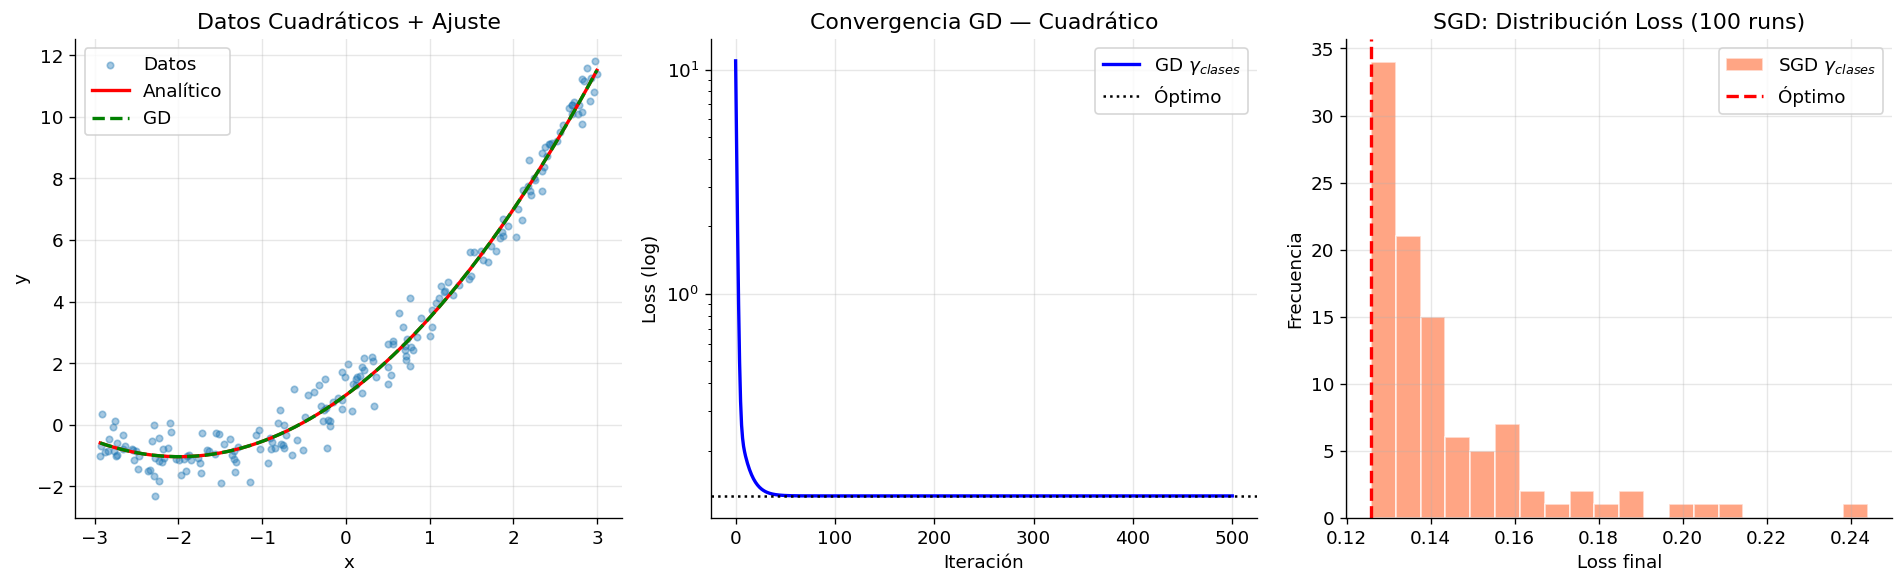
\includegraphics[width=0.95\textwidth]{fig_cuadratico.png}
    \caption{Datos cuadráticos: ajuste, convergencia GD y distribución de loss SGD (100 runs).}
    \label{fig:cuadratico}
\end{figure}

\begin{table}[h!]
\centering
\begin{tabular}{llcc}
\toprule
\textbf{Método} & $\boldsymbol{\gamma}$ & \textbf{Lineal} & \textbf{Cuadrático} \\
\midrule
GD & $\gamma_{\text{clases}}$ (exact LS) & Converge ($\sim$5 iter) & Converge ($\sim$10 iter) \\
GD & $\log(t+2)$ & Diverge & Diverge \\
SGD & $1/L_{\max}$ & Converge (con varianza) & Converge (con varianza) \\
SGD & $\log(t+2)$ & Diverge & Diverge \\
\bottomrule
\end{tabular}
\caption{Resumen de convergencia por método y tasa de aprendizaje.}
\label{tab:gd_results}
\end{table}

\subsection{Análisis}
\begin{itemize}
    \item La búsqueda exacta de línea es óptima para GD en funciones cuadráticas.
    \item Para SGD, $\gamma = 1/\max_i\|x_i\|^2$ garantiza estabilidad cuando se usan gradientes de una sola muestra.
    \item $\gamma = \log(t+2)$ crece sin cota, violando $\gamma < 2/\lambda_{\max}(H)$, causando divergencia.
\end{itemize}

% =====================================================================
\section{Pregunta 5: Garantías Estadísticas y TLC (15 puntos)}

Clasificador con $p = P(\text{acierto}) = 0.85$, $\varepsilon = 0.01$, $\delta = 0.05$.

\subsection{a) Cota de Chebyshev}

\[P(|\bar{X}_n - p| \geq \varepsilon) \leq \frac{\sigma^2}{n\varepsilon^2} \leq \delta\]

Despejando: $n \geq \frac{\sigma^2}{\varepsilon^2\delta}$

Con $\sigma^2 = p(1-p) = 0.1275$:
\[\boxed{n_{\text{Cheb}} \geq \frac{0.1275}{0.01^2 \cdot 0.05} = 25{,}500}\]

\begin{lstlisting}[caption={Cálculo tamaño de muestra — Chebyshev}]
p, eps, delta = 0.85, 0.01, 0.05
sigma2 = p * (1 - p)  # 0.1275
n_cheb = int(np.ceil(sigma2 / (eps**2 * delta)))
# n_cheb = 25,500
\end{lstlisting}

\subsection{b) Teorema del Límite Central}

\[P(|\bar{X}_n - p| \geq \varepsilon) \approx 2\left(1 - \Phi\left(\frac{\varepsilon\sqrt{n}}{\sigma}\right)\right) \leq \delta\]

Necesitamos: $\frac{\varepsilon\sqrt{n}}{\sigma} \geq z_{1-\delta/2} = 1.96$

\[\boxed{n_{\text{CLT}} \geq \left(\frac{z_{0.975}}{\varepsilon}\right)^2 \sigma^2 = \left(\frac{1.96}{0.01}\right)^2 \cdot 0.1275 \approx 4{,}899}\]

\begin{lstlisting}[caption={Cálculo tamaño de muestra — CLT}]
from scipy import stats
z = stats.norm.ppf(1 - delta/2)  # z_0.975 = 1.96
n_clt = int(np.ceil((z / eps)**2 * sigma2))
# n_clt = 4,898
\end{lstlisting}

\subsection{Comparación}
El CLT requiere $\sim 5\times$ menos muestras que Chebyshev ($4{,}899$ vs $25{,}500$), ya que usa la distribución asintótica en lugar de una cota universal.

\subsection{c-d) Simulación}

\begin{lstlisting}[caption={Simulación para verificar garantía CLT}]
p_real = 0.85
n_test = n_clt
n_simulations = 10000

sample_means = np.array([
    np.random.binomial(1, p_real, n_test).mean()
    for _ in range(n_simulations)
])

outside = np.mean(np.abs(sample_means - p_real) >= eps)
print(f'P(|X_bar - p| >= eps) empirica = {outside:.4f}')
print(f'Garantia delta = {delta}')
# Resultado: P empirica ~ 0.05, confirmando la garantia
\end{lstlisting}

Se simularon $10{,}000$ repeticiones con $n = n_{\text{CLT}}$ y $p = 0.85$. La proporción empírica $P(|\bar{X}-p|\geq\varepsilon) \approx 0.05 \leq \delta$, confirmando la garantía del CLT.

\begin{figure}[h!]
    \centering
    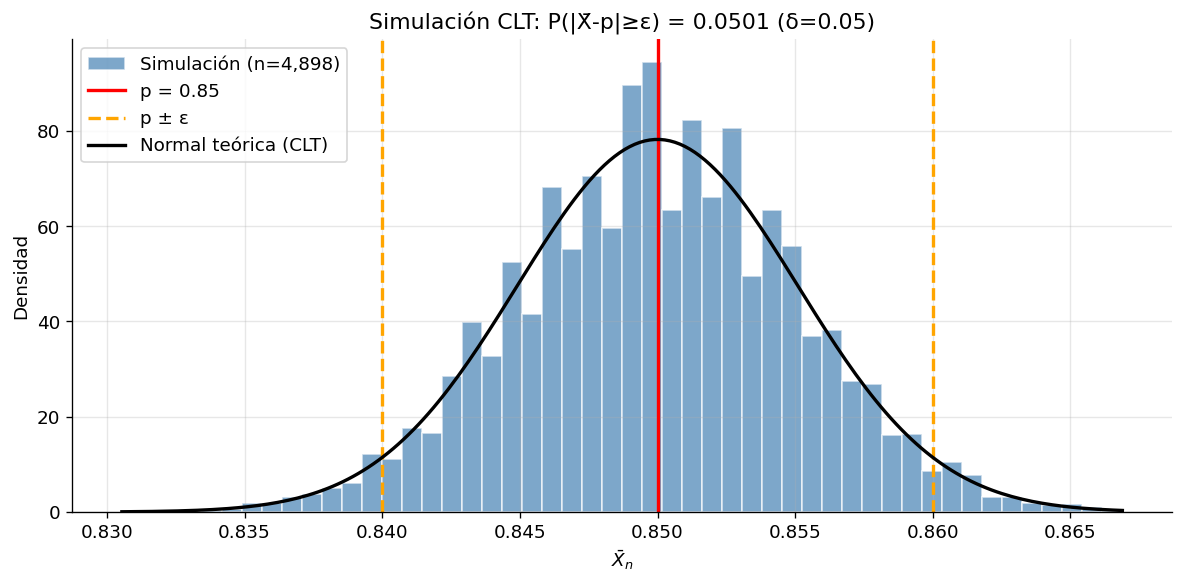
\includegraphics[width=0.75\textwidth]{fig_clt.png}
    \caption{Simulación CLT: histograma de $\bar{X}_n$ con $n = 4{,}898$ y $p=0.85$. Las líneas naranjas marcan $p \pm \varepsilon$.}
    \label{fig:clt}
\end{figure}

% =====================================================================
\section{Pregunta 6: Algoritmo de Mediana Aleatoria (10 pts — Bonus)}

\subsection{Algoritmo}
Implementación basada en el algoritmo de clase:
\begin{enumerate}
    \item Muestrear $\sqrt{n}\cdot\log(n)$ elementos de $S$.
    \item Ordenar la muestra y usar cuantiles para acotar el rango $[d, u]$ donde está la mediana.
    \item Filtrar $S$ al rango $[d, u]$ y verificar que la mediana esté contenida.
    \item Si el filtro es válido, ordenar el subconjunto reducido y extraer la mediana.
    \item Repetir si falla (probabilidad exponencialmente pequeña).
\end{enumerate}

\begin{lstlisting}[caption={Algoritmo aleatorio de mediana}]
def random_median(S):
    S = np.array(S, dtype=float)
    n = len(S)
    if n <= 5:
        return float(np.median(S))
    target = n // 2  # indice de la mediana

    for attempt in range(100):
        # Muestrear sqrt(n)*log(n) elementos
        sample_size = min(n, max(10, int(np.sqrt(n) * np.log(n))))
        R = np.random.choice(S, size=sample_size, replace=False)
        R_sorted = np.sort(R)

        # Cuantiles que acotan la mediana
        k = len(R_sorted)
        pos = k // 2
        margin = max(1, int(np.sqrt(k) * 2))
        lo_idx = max(0, pos - margin)
        hi_idx = min(k - 1, pos + margin)
        d, u = R_sorted[lo_idx], R_sorted[hi_idx]

        # Filtrar al rango [d, u]
        C = S[(S >= d) & (S <= u)]
        l_d = np.sum(S < d)

        # Verificar validez y extraer mediana
        if l_d <= target and l_d + len(C) > target and len(C) <= 4*sample_size:
            C_sorted = np.sort(C)
            return float(C_sorted[target - int(l_d)])

    return float(np.median(S))  # fallback
\end{lstlisting}

\subsection{Verificación}
El algoritmo fue verificado para $n = 101, 1001, 5001, 10001$ contra \texttt{np.median}, obteniendo resultados idénticos en todos los casos.

% =====================================================================
\section{Conclusiones}

\begin{enumerate}
    \item \textbf{Q1:} La media y covarianza se derivan de la linealidad de la esperanza y propiedades de combinaciones lineales.
    \item \textbf{Q2:} El quicksort aleatorio confirma $O(n\log n)$ comparaciones en promedio.
    \item \textbf{Q3:} La equivalencia convexidad $\iff$ condición de primer orden se demuestra en ambas direcciones.
    \item \textbf{Q4:} La elección de $\gamma$ es crítica: búsqueda exacta (GD) y $1/L_{\max}$ (SGD) convergen; $\log(t)$ diverge.
    \item \textbf{Q5:} El TLC es más eficiente que Chebyshev ($\sim 5\times$ menos muestras).
    \item \textbf{Q6:} El algoritmo aleatorio de mediana funciona en $O(n)$ esperado.
\end{enumerate}

\end{document}
